\documentclass[11pt,a4paper]{article}
\usepackage[margin=18mm]{geometry}
\usepackage{amsmath,amssymb,mathtools}
\usepackage{booktabs,array,enumitem}
\usepackage[dvipsnames]{xcolor}
\usepackage{graphicx,listings,tikz,float,needspace}
\usetikzlibrary{arrows.meta,positioning}
\usepackage[most]{tcolorbox}
\usepackage{hyperref}
\hypersetup{colorlinks=true,urlcolor=MidnightBlue,linkcolor=MidnightBlue}
\setlength{\parindent}{0pt}\setlength{\parskip}{4pt}
\newcommand{\course}{PHY4605 Computational Methods in Physics}
\newcommand{\units}[1]{\,\mathrm{#1}}
\newtcolorbox{keybox}{colback=RoyalBlue!5,colframe=RoyalBlue!65!black,boxrule=.7pt,arc=2mm}
\newtcolorbox{checkbox}{colback=ForestGreen!5,colframe=ForestGreen!55!black,boxrule=.7pt,arc=2mm}
\newtcolorbox{aibox}{colback=BurntOrange!7,colframe=BurntOrange!80!black,boxrule=.7pt,arc=2mm}
\lstdefinestyle{matlabstyle}{language=Matlab,basicstyle=\ttfamily\footnotesize,keywordstyle=\color{RoyalBlue!75!black},commentstyle=\color{ForestGreen!55!black},stringstyle=\color{BurntOrange!80!black},numbers=left,numberstyle=\scriptsize\color{black!50},numbersep=5pt,frame=single,rulecolor=\color{RoyalBlue!25},backgroundcolor=\color{RoyalBlue!3},showstringspaces=false,columns=fullflexible,keepspaces=true,breaklines=true}
\begin{document}
{\large\textsc{\course}}\\[-2pt]
{\small Learning Note \textbar\ Week 8}\par\vspace{4pt}
{\LARGE\bfseries ODE Simulation: Euler Steps for Newton Cooling}\par\vspace{3pt}
\textit{Turn a familiar rate law into small, visible temperature updates, then test how timestep size changes the simulation.}

\begin{keybox}\textbf{Physical question.} A hot object cools toward room temperature. Starting at $80\units{^\circ C}$ in a $20\units{^\circ C}$ room, what temperature does an Euler simulation predict from $0$ to $300\units{s}$, and how does the timestep affect confidence in that prediction?\end{keybox}

\section*{Core learning outcomes}
\begin{enumerate}[nosep,leftmargin=5mm]
\item identify the state, rate, initial condition, timestep, and final time in a first-order physical model;
\item trace and complete an Euler update loop that produces a labelled temperature trajectory; and
\item validate the simulation with smaller timesteps, an exact reference, and physical initial-value and trend checks.
\end{enumerate}

\section*{1. A changing state needs a starting value}
The \textbf{state variable} is the object's uniform temperature, $T(t)$. Its value changes with time, so one number is not enough: we need a sequence of temperatures. Newton cooling gives the rate law
\[
\frac{dT}{dt}=-\frac{T-T_{\mathrm{env}}}{\tau}.
\]
Here $T_{\mathrm{env}}=20\units{^\circ C}$ is the constant room temperature and $\tau=100\units{s}$ is a cooling timescale. The initial condition fixes the first state:
\[
T(0)=T_0=80\units{^\circ C}, \qquad 0\le t\le300\units{s}.
\]

The derivative $dT/dt$ is the \textbf{rate of change of temperature}, in $\units{^\circ C\,s^{-1}}$. At $t=0$,
\[
\left.\frac{dT}{dt}\right|_{t=0}
=-\frac{80-20}{100}=-0.6\units{^\circ C\,s^{-1}}.
\]
The negative sign matches the physical prediction: an object warmer than its surroundings cools. The rate becomes smaller in magnitude as $T$ approaches $T_{\mathrm{env}}$.

\begin{checkbox}\textbf{Prediction checkpoint.} For this model, every simulated temperature should begin at $80\units{^\circ C}$, decrease toward $20\units{^\circ C}$, and remain between these values. A result that rises or falls below the room temperature needs investigation.\end{checkbox}

\section*{2. Euler uses the current rate for one short step}
Choose a timestep $h$, measured in seconds. Euler's method replaces the continuous change during one timestep by the current rate multiplied by the timestep:
\[
T_{n+1}=T_n+h\left(-\frac{T_n-T_{\mathrm{env}}}{\tau}\right).
\]
Read this from left to right: start with the current temperature $T_n$, calculate its cooling rate, then add \textit{rate $\times$ timestep} to obtain the next temperature $T_{n+1}$. The product has the correct unit:
\[
\units{^\circ C\,s^{-1}}\times\units{s}=\units{^\circ C}.
\]

The method needs a sequence of times, a first temperature from the initial condition, and one update for each adjacent pair of times. It does not solve the differential equation symbolically; it constructs a numerical approximation step by step.

\section*{3. Trace the first two Euler updates}
Use the deliberately coarse starting timestep $h=50\units{s}$. The first rate is $-0.6\units{^\circ C\,s^{-1}}$, so
\[
T_1=80+50(-0.6)=50\units{^\circ C}.
\]
At $t=50\units{s}$ the object is still warmer than the room. Its new rate is
\[
-\frac{50-20}{100}=-0.3\units{^\circ C\,s^{-1}},
\]
so the second update is
\[
T_2=50+50(-0.3)=35\units{^\circ C}.
\]

\begin{center}\small
\begin{tabular}{rrrr}
\toprule
step $n$ & $t_n$ (s) & $T_n$ ($^\circ$C) & rate at $T_n$ ($^\circ$C s$^{-1}$)\\
\midrule
0 & 0 & 80 & $-0.60$\\
1 & 50 & 50 & $-0.30$\\
2 & 100 & 35 & $-0.15$\\
\bottomrule
\end{tabular}
\end{center}

\begin{aibox}\textbf{A common physical/logical defect.} In the update, use the \emph{current} value $T_n$ on the right-hand side. Reusing $T_0$ at every step would apply the original cooling rate repeatedly, even after the object has cooled. MATLAB can run that code, but the physics would be wrong.\end{aibox}

\section*{4. Pseudocode before MATLAB}
\begin{enumerate}[nosep,leftmargin=7mm]
\item state the environment temperature, initial temperature, timescale, timestep, and final time with units;
\item create all time positions from $0$ to the final time using the chosen timestep;
\item reserve one temperature value for every time position, then place the initial condition in the first position;
\item for each current position, calculate the cooling rate from the current temperature;
\item use Euler's update rule to store the next temperature;
\item plot temperature against time with axis labels and units; and
\item check the initial value and trend, then compare the result with a smaller timestep and a reference.
\end{enumerate}

\Needspace{28\baselineskip}
\section*{5. A commented Euler-loop scaffold}
The loop counter \texttt{n} labels the \emph{current} position. MATLAB uses one-based indexing, so the current temperature is \texttt{T\_C(n)} and the next position is \texttt{T\_C(n+1)}.

\begin{lstlisting}[style=matlabstyle]
T_room_C = 20;
T_initial_C = 80;
tau_s = 100;
dt_s = 50;
t_final_s = 300;

nSteps = t_final_s / dt_s;
t_s = (0:nSteps) * dt_s;
T_C = zeros(size(t_s));
T_C(1) = T_initial_C;       % initial condition at t = 0

for n = 1:nSteps
    rate_C_per_s = -(T_C(n) - T_room_C) / tau_s;
    T_C(n+1) = T_C(n) + dt_s * rate_C_per_s;
end

plot(t_s,T_C,'o-','LineWidth',1.2)
xlabel('Time, t (s)')
ylabel('Temperature, T (degrees Celsius)')
grid on
\end{lstlisting}

Before running, trace the first two loop passes against the table above. Then change only \texttt{dt\_s} to $25\units{s}$ or $12.5\units{s}$ and predict what will happen to the plotted points and the final temperature.

\section*{6. Timestep comparison and an independent reference}
For this teaching model only, a supplied exact solution provides an independent reference:
\[
T_{\mathrm{exact}}(t)=20+60e^{-t/100}.
\]
It gives $T_{\mathrm{exact}}(300\units{s})=22.9872\units{^\circ C}$. The figure compares this continuous reference with Euler simulations. \textit{Accessibility description: a black smooth cooling curve falls from $80\units{^\circ C}$ toward the dashed $20\units{^\circ C}$ room-temperature line. Euler points using smaller timesteps lie progressively closer to the black curve.}

\begin{figure}[H]
\centering
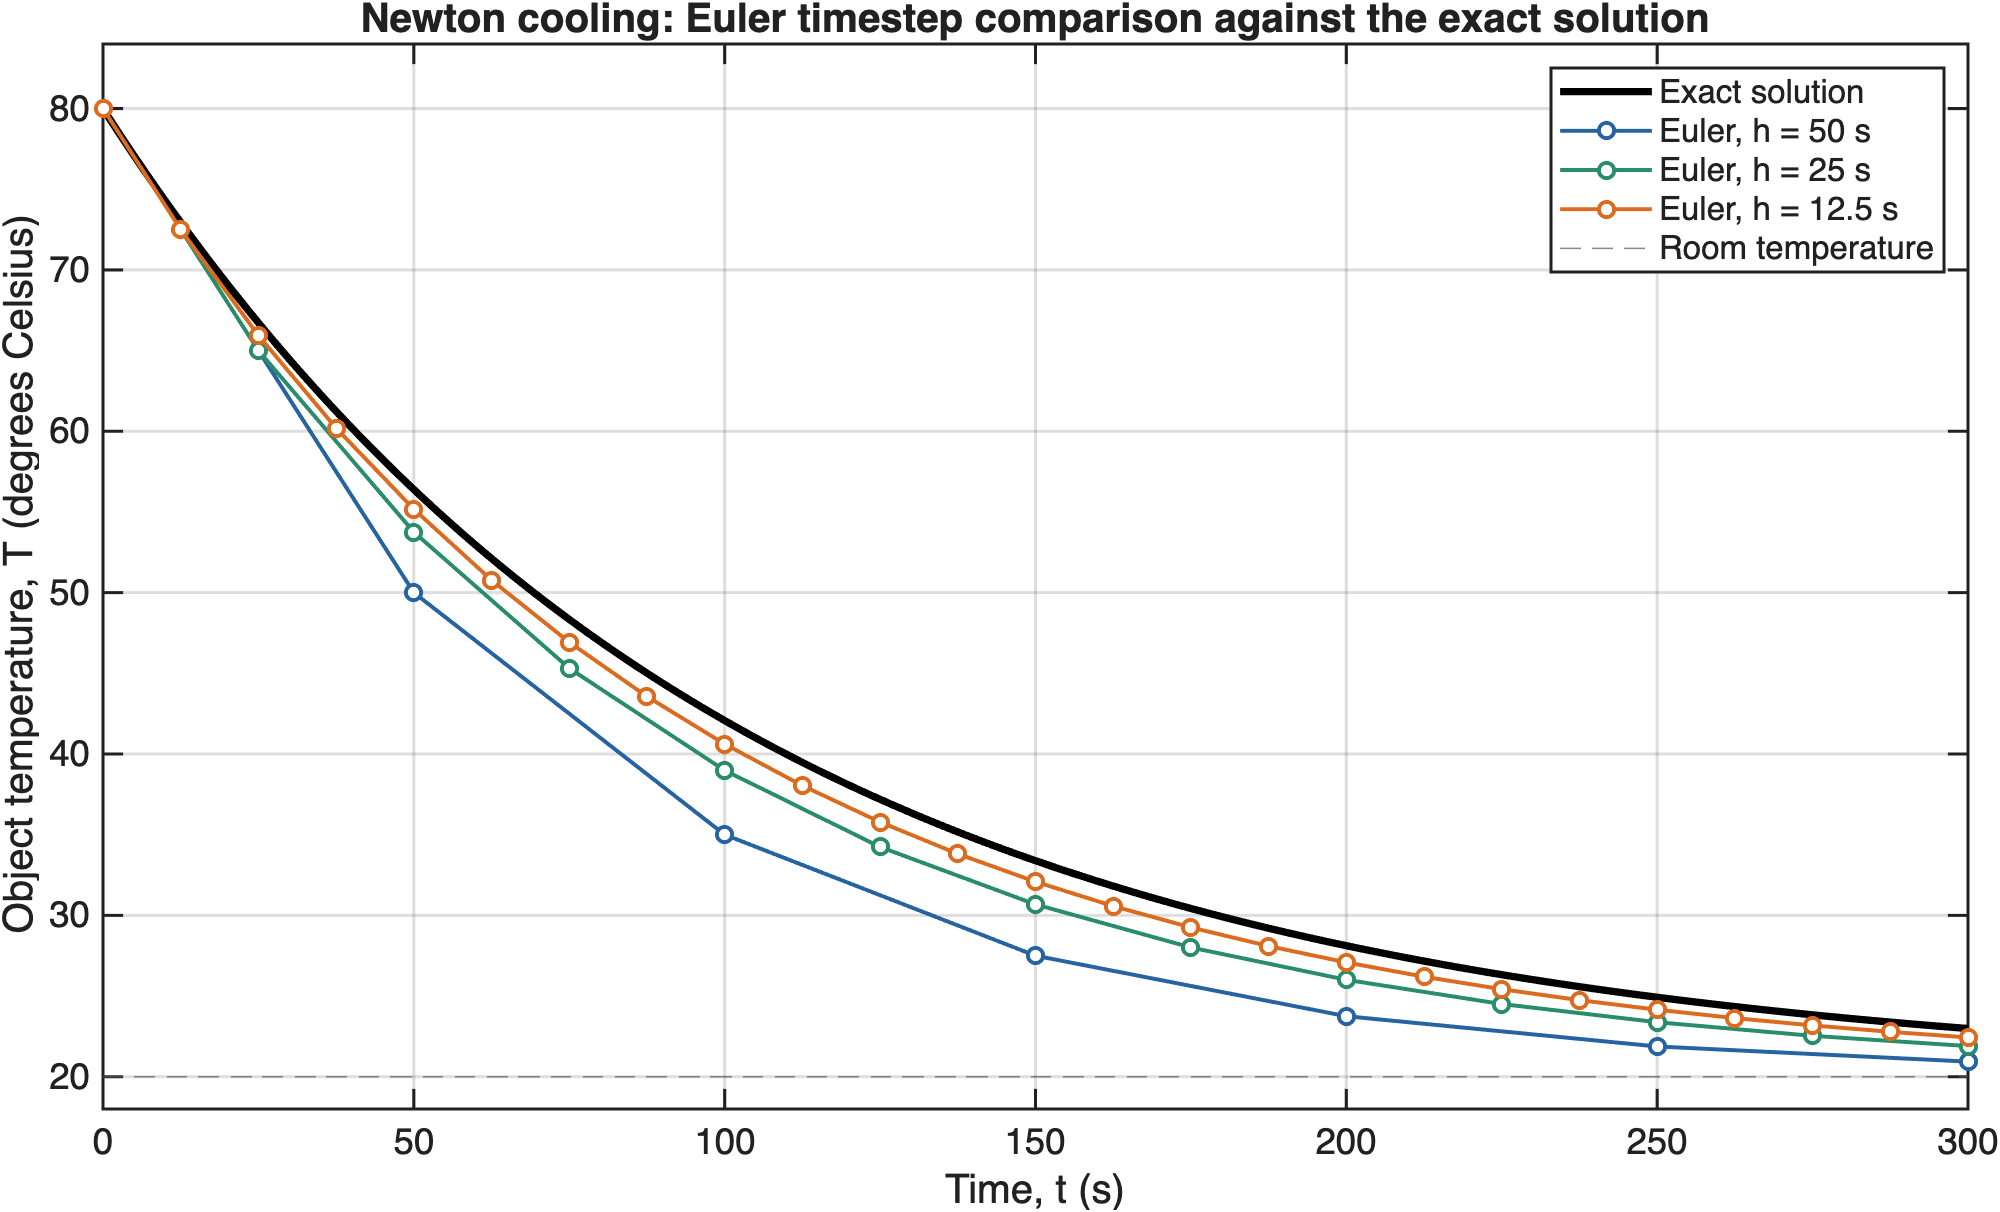
\includegraphics[width=.91\linewidth]{assets/week08_newton_cooling_euler_comparison.png}
\caption{Newton cooling from $80\units{^\circ C}$ toward a $20\units{^\circ C}$ environment. Euler trajectories use $h=50$, $25$, and $12.5\units{s}$; the black line is the supplied exact reference.}
\end{figure}

\begin{center}\small
\begin{tabular}{rrrr}
\toprule
$h$ (s) & Euler $T(300\units{s})$ ($^\circ$C) & abs. error ($^\circ$C) & comparison\\
\midrule
50.0 & 20.9375 & 2.0497 & coarsest supplied result\\
25.0 & 21.9006 & 1.0866 & closer to reference\\
12.5 & 22.4341 & 0.5531 & closest supplied result\\
\bottomrule
\end{tabular}
\end{center}

The physics and final time are unchanged across the rows. Only $h$ changes. For these supplied steps, smaller timesteps give endpoint values closer to the reference. This is evidence about this model and interval, rather than a guarantee that every timestep is acceptable for every ODE.

\section*{7. Core validation: check the start, the trend, and the reference}
The Euler trajectory with $h=50\units{s}$ starts at the required $80\units{^\circ C}$, and its first two calculated values are $50\units{^\circ C}$ and $35\units{^\circ C}$, as traced by hand. Every plotted trajectory decreases toward the $20\units{^\circ C}$ environment and remains within the physical bounds for this case.

\begin{checkbox}\textbf{Validation statement.} At the same final time, the endpoint error decreases from $2.0497\units{^\circ C}$ for $h=50\units{s}$ to $0.5531\units{^\circ C}$ for $h=12.5\units{s}$. Together with the correct initial value and cooling trend, this supports the finer Euler result for the stated Newton-cooling model.\end{checkbox}

\section*{8. Interpret the simulated trajectory}
Temperature falls quickly at first because the difference $T-T_{\mathrm{env}}$ is large. As the object approaches the room temperature, the magnitude of the rate decreases, so the curve flattens. At $300\units{s}$, the exact model predicts about $23.0\units{^\circ C}$: the object is close to, but has not reached, the environment temperature.

The numerical result is only as appropriate as its physical model. Here we assumed a constant environment temperature and one constant cooling timescale. Changing airflow, contact with another object, or internal heat generation could make that assumption unsuitable.

\section*{Working exposure: supplied \texttt{ode45} reference}
MATLAB's \texttt{ode45} is a solver that can produce a reference trajectory without writing the Euler loop. Read the supplied call as evidence, but Core work remains the visible Euler update and its validation:
\begin{lstlisting}[style=matlabstyle]
coolingRate = @(t,T) -(T - T_room_C) / tau_s;
[t45_s,T45_C] = ode45(coolingRate,[0 t_final_s],T_initial_C);
plot(t45_s,T45_C,'k-')
\end{lstlisting}
The anonymous function states the same rate law. The interval \texttt{[0 t\_final\_s]} and initial condition \texttt{T\_initial\_C} remain physical inputs that must be checked.

\section*{Optional stretch}
Optional extensions include deriving formal Euler stability conditions, comparing Runge--Kutta methods, simulating a stiff system, handling events, or coupling several nonlinear ODEs. These are not required for the Core pathway.

\section*{Three takeaways}
\begin{enumerate}[nosep,leftmargin=6mm]
\item A first-order ODE simulation needs a state, a rate law, an initial condition, a timestep, and a final time with units.
\item Euler updates the next state from the current state and current rate; trace the first steps before trusting a loop.
\item Compare timesteps with an independent reference and test the initial value and physical trend before interpreting a numerical trajectory.
\end{enumerate}

\begin{keybox}\textbf{Preparation for the practical.} For each supplied ODE context, identify the state and rate, label the initial condition and units, trace two Euler steps, then record an initial-value/trend check plus a timestep or reference comparison before explaining the output.\end{keybox}
\end{document}
